\documentclass[9pt]{beamer}
\usetheme{cmepda}

\usepackage[utf8]{inputenc}
\usepackage[T1]{fontenc}

\graphicspath{{figures/}} 


\title{Advanced python features}
\subtitle{Computing Methods for Experimental Physics and Data Analysis}
\date{Compiled on \today}
\author{A. Manfreda}
\institute[INFN]{INFN--Pisa}
\email{alberto.manfreda@pi.infn.it}


\begin{document}


\titleframe


\begin{frame}
  \frametitle{Errors and Exceptions}
  
  \begin{itemize}
    \item \alert{Error handling} is one of the most important problem to solve when designing a program
    \item What should I do when I piece of code fails?
    \item What does fail mean?
    \begin {itemize}
      \item Invalid input e.g. passing a path to a non existent file, or passing a string to a function for dividing numbers
      \item Valid output not found, e.g searching the position of the letter 'd' in the string 'elephant'
      \item Output cannot be find in a reasonable amount of time
      \item Runtime resource failures: network connection down, disk space ended\dots
    \end{itemize}
    \item Two phylosophies (historically):
    \begin{itemize}
      \item Return some \alert{error flag} (in different ways) to tell the user that something went wrong
      \item \alert{Exceptions}
    \end{itemize}
    \item Example: a typical convention for programs is to return 0 from the main if the execution was successful and an
          error code (integer number) otherwise
  \end{itemize}
  
\end{frame}


\begin{frame}
  \frametitle{Error flags}
  \begin{Verbatim}[label=\makebox{\url{https://github.com/lucabaldini/cmepda/tree/master/slides/latex/snippets/error\_flags.py}},commandchars=\\\{\}]
\PY{c+c1}{\PYZsh{} The \PYZsq{}find()\PYZsq{} method for strings in python uses an error flag}
\PY{n}{text} \PY{o}{=} \PY{l+s+s1}{\PYZsq{}}\PY{l+s+s1}{elephant}\PY{l+s+s1}{\PYZsq{}}
\PY{k}{print}\PY{p}{(}\PY{n}{text}\PY{o}{.}\PY{n}{find}\PY{p}{(}\PY{l+s+s1}{\PYZsq{}}\PY{l+s+s1}{p}\PY{l+s+s1}{\PYZsq{}}\PY{p}{)}\PY{p}{)} \PY{c+c1}{\PYZsh{} upon success returns the position of the substring}
\PY{k}{print}\PY{p}{(}\PY{n}{text}\PY{o}{.}\PY{n}{find}\PY{p}{(}\PY{l+s+s1}{\PYZsq{}}\PY{l+s+s1}{d}\PY{l+s+s1}{\PYZsq{}}\PY{p}{)}\PY{p}{)} \PY{c+c1}{\PYZsh{} returns \PYZhy{}1 if the substring is not found}

\PY{k}{def} \PY{n+nf}{safe\PYZus{}division}\PY{p}{(}\PY{n}{a}\PY{p}{,} \PY{n}{b}\PY{p}{)}\PY{p}{:}
    \PY{k}{if} \PY{n}{b} \PY{o}{==} \PY{l+m+mi}{0}\PY{p}{:}
        \PY{k}{return} \PY{l+m+mi}{0} \PY{c+c1}{\PYZsh{} Is that meaningful? What can we return?}
    \PY{k}{else}\PY{p}{:}
        \PY{k}{return} \PY{n}{a}\PY{o}{/}\PY{n}{b}

\PY{c+c1}{\PYZsh{} Why is this dangerous?}
\PY{n}{num\PYZus{}process} \PY{o}{=} \PY{l+m+mi}{0}
\PY{n}{num\PYZus{}cpu\PYZus{}available} \PY{o}{=} \PY{l+m+mi}{3}
\PY{n}{average\PYZus{}cpu\PYZus{}available} \PY{o}{=} \PY{n}{safe\PYZus{}division}\PY{p}{(}\PY{n}{num\PYZus{}cpu\PYZus{}available}\PY{p}{,} \PY{n}{num\PYZus{}process}\PY{p}{)}
\PY{k}{print}\PY{p}{(}\PY{n}{average\PYZus{}cpu\PYZus{}available}\PY{p}{)} \PY{c+c1}{\PYZsh{} Oops no cpu available... or not?}

[Output]
3
-1
0
\end{Verbatim}
\end{frame}


\begin{frame}
  \frametitle{Problems of error flags}
  
    Error codes have their use (and are fine in some cases) but they suffer from a few issues:
    \begin{itemize}
      \item Choosing them is often arbitrary (and sometimes is difficult to make a sensible choice)
      \begin{itemize}
        \item What if all the numbers can represent meaningful output of the function?
      \end{itemize}
      \item Are cumbersome to use
      \begin{itemize}
        \item Which error flag is used by a function? 0? -1? 99999999? $\rightarrow$ you have to go through the documentation for each!
        \item If you have a deep hierarchy of functions you have to perform checks and pass the error up at every level!
      \end{itemize}
      \item What if the caller of a function does not check the error flag?
      \begin{itemize}
        \item The bug can propagate \alert{silently} through its code!
      \end{itemize}
    \end{itemize}
   
    \medskip
   
    We want something that:
    \begin{itemize}
      \item Is clearly separated from the returned output
      \item Cannot be silently ignored by the user
      \item Is easy to report to upper level without lots of lines of code
    \end{itemize}
  
\end{frame}


\begin{frame}
  \frametitle{Enter exceptions}

  \begin{itemize}
    \item An exception is an object that can be \alert{raised} (in other languages also \textit{thrown}) by
          a piece of code to signal that something went wrong
    \item When an exception is raised the normal flow of the code is interrupted
    \item The program automatically propagate the exception back in the function hierarchy
          until it found a place where the exception is  \alert{catched} and handled
    \item If the exception is never catched, not even in the main, the program crash \alert{with a specific error message}
    \item Cathcing the exception is done with a \emph{try - except} block
  \end{itemize}
\end{frame}


\begin{frame}
  \frametitle{Exceptions}
  \begin{Verbatim}[label=\makebox{\url{https://github.com/lucabaldini/cmepda/tree/master/slides/latex/snippets/exceptions.py}},commandchars=\\\{\}]
\PY{k}{def} \PY{n+nf}{throwing\PYZus{}function}\PY{p}{(}\PY{p}{)}\PY{p}{:}
    \PY{k}{raise}
    \PY{k}{print}\PY{p}{(}\PY{l+s+s2}{\PYZdq{}}\PY{l+s+s2}{This line is never executed!}\PY{l+s+s2}{\PYZdq{}}\PY{p}{)}

\PY{k}{try}\PY{p}{:}
  \PY{n}{throwing\PYZus{}function}\PY{p}{(}\PY{p}{)}
  \PY{k}{print}\PY{p}{(}\PY{l+s+s2}{\PYZdq{}}\PY{l+s+s2}{This line is never executed as well!}\PY{l+s+s2}{\PYZdq{}}\PY{p}{)}
\PY{k}{except}\PY{p}{:}
  \PY{k}{print}\PY{p}{(}\PY{l+s+s2}{\PYZdq{}}\PY{l+s+s2}{This line is executed only if an exception is raised in the try block}\PY{l+s+s2}{\PYZdq{}}\PY{p}{)}
\PY{k}{else}\PY{p}{:} \PY{c+c1}{\PYZsh{} optional!}
  \PY{k}{print}\PY{p}{(}\PY{l+s+s2}{\PYZdq{}}\PY{l+s+s2}{This line is executed only if no exception is raised in the try block}\PY{l+s+s2}{\PYZdq{}}\PY{p}{)}
\PY{k}{finally}\PY{p}{:} \PY{c+c1}{\PYZsh{} optional!}
  \PY{k}{print}\PY{p}{(}\PY{l+s+s2}{\PYZdq{}}\PY{l+s+s2}{This line is always executed}\PY{l+s+s2}{\PYZdq{}}\PY{p}{)}

[Output]
This line is executed only if an exception is raised in the try block
This line is always executed
\end{Verbatim}
\end{frame}


\begin{frame}
  \frametitle{The beauty of throwning stuff}

  \begin{itemize}
    \item If that was all, exceptions would only be moderately useful
    \item The real bargain is that you can send back information together with the exception
    \item In fact you \textit{are sending a full object}: the excetpion iteslf. Surprised?
    \item Inside the exception you can report all kind of data useful to reconstruct the exact error,
          which can be used by the caller for debug or to produce meaningful error messages
    \item You can also select which exceptions you catch, leaving the others propagate up
    \item Python provides a rich hierarchy of exception classes, which you can further customize
          (if you want) by deriving your own subclasses
  \end{itemize}
\end{frame}


\begin{frame}
  \frametitle{The family tree of Python exceptions}
  \centering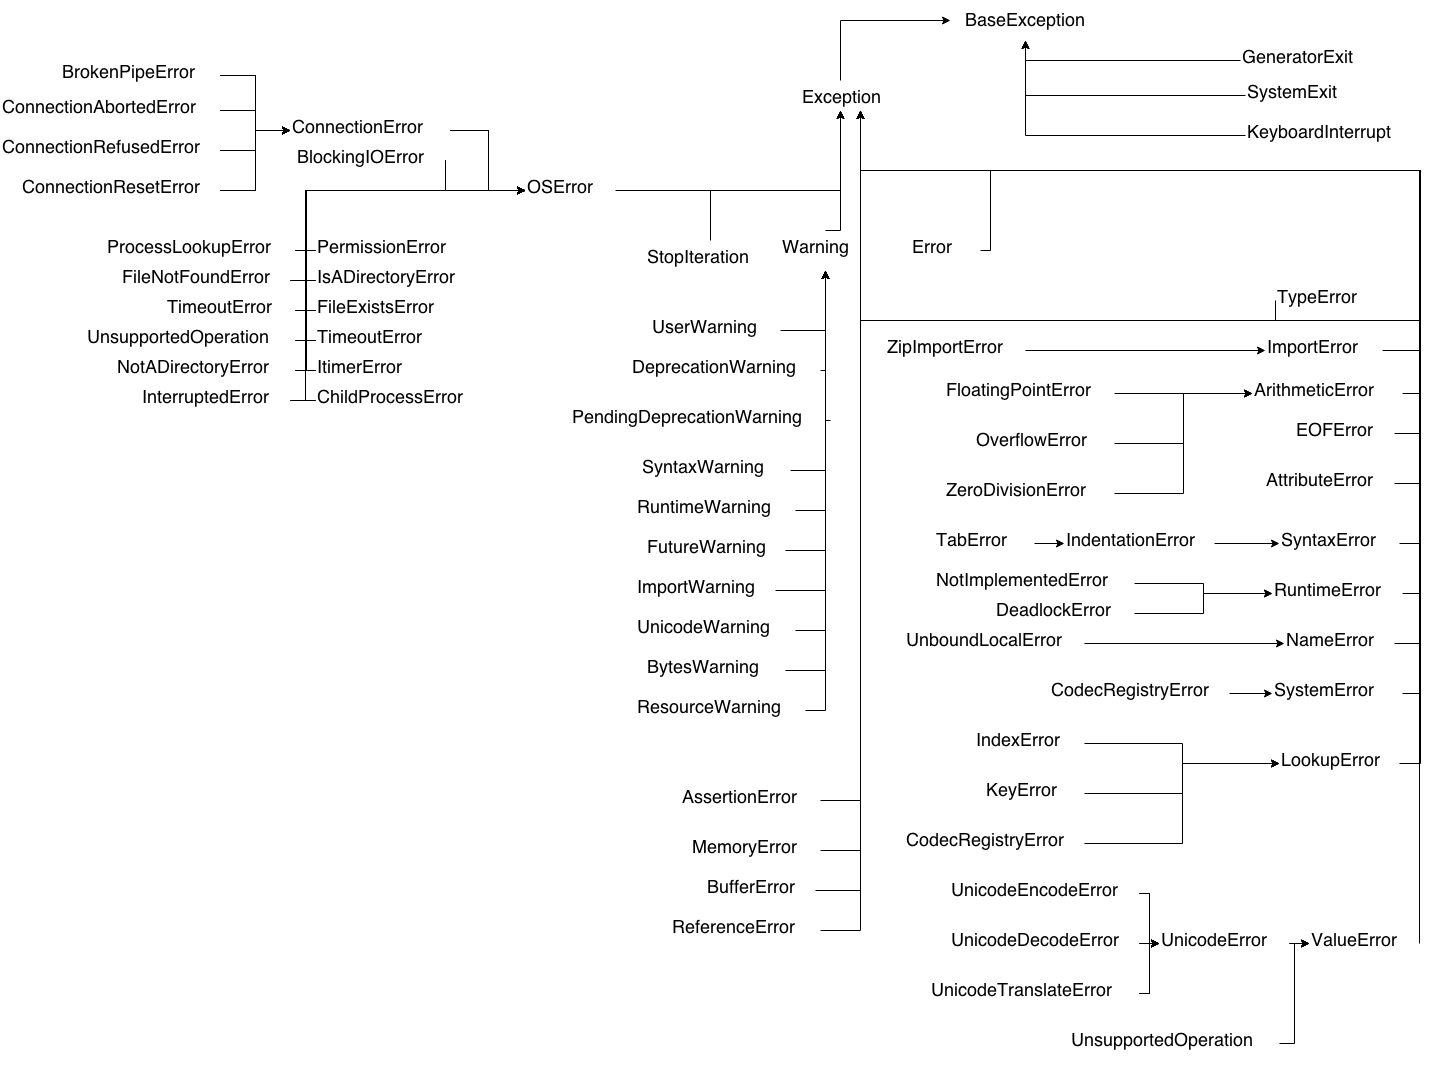
\includegraphics[height=0.8\textheight]{python_exceptions}
\end{frame}


\begin{frame}
  \frametitle{Catching exceptions}
  \begin{Verbatim}[label=\makebox{\url{https://github.com/lucabaldini/cmepda/tree/master/slides/latex/snippets/try\_block.py}},commandchars=\\\{\}]
\PY{k}{try}\PY{p}{:}
    \PY{k}{with} \PY{n+nb}{open} \PY{p}{(}\PY{l+s+s1}{\PYZsq{}}\PY{l+s+s1}{i\PYZus{}do\PYZus{}not\PYZus{}exist.txt}\PY{l+s+s1}{\PYZsq{}}\PY{p}{)} \PY{k}{as} \PY{n}{lab\PYZus{}data\PYZus{}file}\PY{p}{:}
        \PY{l+s+sd}{\PYZdq{}\PYZdq{}\PYZdq{} Do some process here...}
\PY{l+s+sd}{        \PYZdq{}\PYZdq{}\PYZdq{}}
        \PY{k}{pass}
        
\PY{k}{except} \PY{n}{FileNotFoundError} \PY{k}{as} \PY{n}{e}\PY{p}{:} \PY{c+c1}{\PYZsh{} we assign a name to the the exception }
    \PY{k}{print}\PY{p}{(}\PY{n}{e}\PY{p}{)}

\PY{c+c1}{\PYZsh{} We can be less specific by catching a parent exception}
\PY{k}{except} \PY{n+ne}{OSError} \PY{k}{as} \PY{n}{e}\PY{p}{:} \PY{c+c1}{\PYZsh{} OSError is a parent class of FileNotFoundError}
    \PY{k}{print}\PY{p}{(}\PY{n}{e}\PY{p}{)}

\PY{c+c1}{\PYZsh{} catching Exception will catch almost everything!}
\PY{k}{except} \PY{n+ne}{Exception} \PY{k}{as} \PY{n}{e}\PY{p}{:}
    \PY{k}{print}\PY{p}{(}\PY{n}{e}\PY{p}{)}

[Output]
[Errno 2] No such file or directory: 'i_do_not_exist.txt'
\end{Verbatim}
\end{frame}


\begin{frame}
  \frametitle{Throwing exceptions}
  \begin{Verbatim}[label=\makebox{\url{https://github.com/lucabaldini/cmepda/tree/master/slides/latex/snippets/throwing.py}},commandchars=\\\{\}]
\PY{k}{def} \PY{n+nf}{throwing\PYZus{}function}\PY{p}{(}\PY{p}{)}\PY{p}{:}
    \PY{c+c1}{\PYZsh{} You can pass useful message to the exceptions you throw}
    \PY{k}{raise} \PY{n+ne}{RuntimeError}\PY{p}{(}\PY{l+s+s1}{\PYZsq{}}\PY{l+s+s1}{this is a useful debug text}\PY{l+s+s1}{\PYZsq{}}\PY{p}{)} 

\PY{k}{try}\PY{p}{:}
    \PY{n}{throwing\PYZus{}function}\PY{p}{(}\PY{p}{)}
\PY{k}{except} \PY{n+ne}{RuntimeError} \PY{k}{as} \PY{n}{e}\PY{p}{:}
    \PY{c+c1}{\PYZsh{} The message can be retrieved by printing the exception}
    \PY{k}{print}\PY{p}{(}\PY{n}{e}\PY{p}{)}

[Output]
this is a useful debug text
\end{Verbatim}
\end{frame}


\begin{frame}
  \frametitle{Where to catch exceptions?}

  \begin{itemize}
    \item Differently from error flags, which needs to be checked as early as
          possible, you are not in a rush with exceptions
    \item Remeber: your goal is to provide the user a meaningful error message and
          useful debug information.
    \item You should catch an exception only when you have enough context to
          do that - which sometimes means waiting a few levels in the hierarchy!
  \end{itemize}
\end{frame}


\begin{frame}
  \frametitle{When to catch?}
  \centering
  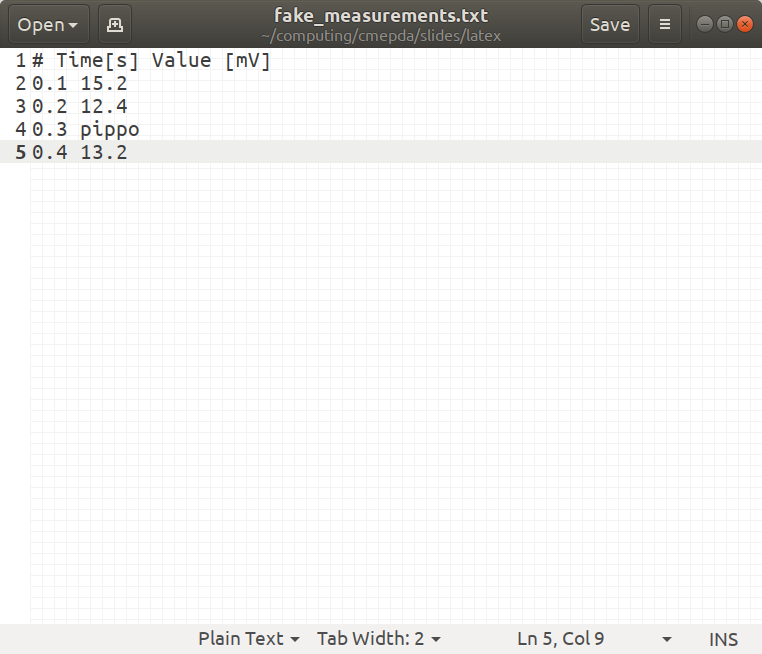
\includegraphics[width=0.8\textwidth]{lab_file.png}
\end{frame}



\begin{frame}
  \frametitle{When to catch?}
  \begin{Verbatim}[label=\makebox{\url{https://github.com/lucabaldini/cmepda/tree/master/slides/latex/snippets/when\_to\_catch.py}},commandchars=\\\{\}]
\PY{k}{def} \PY{n+nf}{parse\PYZus{}line}\PY{p}{(}\PY{n}{line}\PY{p}{)}\PY{p}{:}
    \PY{l+s+sd}{\PYZdq{}\PYZdq{}\PYZdq{} Parse a line of the file and return the values as float\PYZdq{}\PYZdq{}\PYZdq{}}
    \PY{n}{values} \PY{o}{=} \PY{n}{line}\PY{o}{.}\PY{n}{strip}\PY{p}{(}\PY{l+s+s1}{\PYZsq{}}\PY{l+s+se}{\PYZbs{}n}\PY{l+s+s1}{\PYZsq{}}\PY{p}{)}\PY{o}{.}\PY{n}{split}\PY{p}{(}\PY{l+s+s1}{\PYZsq{}}\PY{l+s+s1}{ }\PY{l+s+s1}{\PYZsq{}}\PY{p}{)}
    \PY{c+c1}{\PYZsh{} the following two lines may generate exceptions if they fails!}
    \PY{n}{time} \PY{o}{=} \PY{n+nb}{float}\PY{p}{(}\PY{n}{values}\PY{p}{[}\PY{l+m+mi}{0}\PY{p}{]}\PY{p}{)}
    \PY{n}{tension} \PY{o}{=} \PY{n+nb}{float}\PY{p}{(}\PY{n}{values}\PY{p}{[}\PY{l+m+mi}{1}\PY{p}{]}\PY{p}{)}
    \PY{k}{return} \PY{n}{time}\PY{p}{,} \PY{n}{tension}

\PY{k}{with} \PY{n+nb}{open}\PY{p}{(}\PY{l+s+s1}{\PYZsq{}}\PY{l+s+s1}{snippets/data/fake\PYZus{}measurements.txt}\PY{l+s+s1}{\PYZsq{}}\PY{p}{)} \PY{k}{as} \PY{n}{lab\PYZus{}data\PYZus{}file}\PY{p}{:}
    \PY{k}{for} \PY{n}{line} \PY{o+ow}{in} \PY{n}{lab\PYZus{}data\PYZus{}file}\PY{p}{:}
        \PY{k}{if} \PY{o+ow}{not} \PY{n}{line}\PY{o}{.}\PY{n}{startswith}\PY{p}{(}\PY{l+s+s1}{\PYZsq{}}\PY{l+s+s1}{\PYZsh{}}\PY{l+s+s1}{\PYZsq{}}\PY{p}{)}\PY{p}{:} \PY{c+c1}{\PYZsh{} skip comments}
            \PY{n}{time}\PY{p}{,} \PY{n}{tension} \PY{o}{=} \PY{n}{parse\PYZus{}line}\PY{p}{(}\PY{n}{line}\PY{p}{)}
            \PY{k}{print}\PY{p}{(}\PY{n}{time}\PY{p}{,} \PY{n}{tension}\PY{p}{)}

[Output]
0.1 15.2
0.2 12.4
Traceback (most recent call last):
  File "snippets/when_to_catch.py", line 12, in <module>
    time, tension = parse_line(line)
  File "snippets/when_to_catch.py", line 6, in parse_line
    tension = float(values[1])
ValueError: could not convert string to float: 'pippo'
\end{Verbatim}
\end{frame}


\begin{frame}
  \frametitle{Catch too early}
  \begin{Verbatim}[label=\makebox{\url{https://github.com/lucabaldini/cmepda/tree/master/slides/latex/snippets/when\_to\_catch\_1.py}},commandchars=\\\{\}]
\PY{k}{def} \PY{n+nf}{parse\PYZus{}line}\PY{p}{(}\PY{n}{line}\PY{p}{)}\PY{p}{:}
    \PY{l+s+sd}{\PYZdq{}\PYZdq{}\PYZdq{} Parse a line of the file and return the values as float\PYZdq{}\PYZdq{}\PYZdq{}}
    \PY{n}{values} \PY{o}{=} \PY{n}{line}\PY{o}{.}\PY{n}{strip}\PY{p}{(}\PY{l+s+s1}{\PYZsq{}}\PY{l+s+se}{\PYZbs{}n}\PY{l+s+s1}{\PYZsq{}}\PY{p}{)}\PY{o}{.}\PY{n}{split}\PY{p}{(}\PY{l+s+s1}{\PYZsq{}}\PY{l+s+s1}{ }\PY{l+s+s1}{\PYZsq{}}\PY{p}{)}
    \PY{k}{try}\PY{p}{:}
        \PY{n}{time} \PY{o}{=} \PY{n+nb}{float}\PY{p}{(}\PY{n}{values}\PY{p}{[}\PY{l+m+mi}{0}\PY{p}{]}\PY{p}{)}
        \PY{n}{tension} \PY{o}{=} \PY{n+nb}{float}\PY{p}{(}\PY{n}{values}\PY{p}{[}\PY{l+m+mi}{1}\PY{p}{]}\PY{p}{)}
    \PY{k}{except} \PY{n+ne}{ValueError} \PY{k}{as} \PY{n}{e}\PY{p}{:}
        \PY{k}{print}\PY{p}{(}\PY{n}{e}\PY{p}{)} \PY{c+c1}{\PYZsh{} This is not useful \PYZhy{} which line of the file has the error?}
        \PY{k}{return} \PY{n+nb+bp}{None} \PY{c+c1}{\PYZsh{} We can\PYZsq{}t really return something meaningful}
    \PY{k}{return} \PY{n}{time}\PY{p}{,} \PY{n}{tension}

\PY{k}{with} \PY{n+nb}{open}\PY{p}{(}\PY{l+s+s1}{\PYZsq{}}\PY{l+s+s1}{measurements.txt}\PY{l+s+s1}{\PYZsq{}}\PY{p}{)} \PY{k}{as} \PY{n}{lab\PYZus{}data\PYZus{}file}\PY{p}{:}
    \PY{k}{for} \PY{n}{line} \PY{o+ow}{in} \PY{n}{lab\PYZus{}data\PYZus{}file}\PY{p}{:}
        \PY{k}{if} \PY{o+ow}{not} \PY{n}{line}\PY{o}{.}\PY{n}{startswith}\PY{p}{(}\PY{l+s+s1}{\PYZsq{}}\PY{l+s+s1}{\PYZsh{}}\PY{l+s+s1}{\PYZsq{}}\PY{p}{)}\PY{p}{:} \PY{c+c1}{\PYZsh{} skip comments}
            \PY{n}{time}\PY{p}{,} \PY{n}{tension} \PY{o}{=} \PY{n}{parse\PYZus{}line}\PY{p}{(}\PY{n}{line}\PY{p}{)}
            \PY{k}{print}\PY{p}{(}\PY{n}{time}\PY{p}{,} \PY{n}{tension}\PY{p}{)} \PY{c+c1}{\PYZsh{} This line still crash badly!}

[Output]
0.1 15.2
0.2 12.4
could not convert string to float: 'pippo'
Traceback (most recent call last):
  File "snippets/when_to_catch_1.py", line 15, in <module>
    time, tension = parse_line(line)
TypeError: 'NoneType' object is not iterable
\end{Verbatim}
\end{frame}


\begin{frame}
  \frametitle{Catch when needed}
  \begin{Verbatim}[label=\makebox{\url{https://github.com/lucabaldini/cmepda/tree/master/slides/latex/snippets/when\_to\_catch\_2.py}},commandchars=\\\{\}]
\PY{k}{def} \PY{n+nf}{parse\PYZus{}line}\PY{p}{(}\PY{n}{line}\PY{p}{)}\PY{p}{:}
    \PY{l+s+sd}{\PYZdq{}\PYZdq{}\PYZdq{} Parse a line of the file and return the values as float\PYZdq{}\PYZdq{}\PYZdq{}}
    \PY{n}{values} \PY{o}{=} \PY{n}{line}\PY{o}{.}\PY{n}{strip}\PY{p}{(}\PY{l+s+s1}{\PYZsq{}}\PY{l+s+se}{\PYZbs{}n}\PY{l+s+s1}{\PYZsq{}}\PY{p}{)}\PY{o}{.}\PY{n}{split}\PY{p}{(}\PY{l+s+s1}{\PYZsq{}}\PY{l+s+s1}{ }\PY{l+s+s1}{\PYZsq{}}\PY{p}{)}
    \PY{c+c1}{\PYZsh{} the following two lines may generate exceptions if they fails!}
    \PY{n}{time} \PY{o}{=} \PY{n+nb}{float}\PY{p}{(}\PY{n}{values}\PY{p}{[}\PY{l+m+mi}{0}\PY{p}{]}\PY{p}{)}
    \PY{n}{tension} \PY{o}{=} \PY{n+nb}{float}\PY{p}{(}\PY{n}{values}\PY{p}{[}\PY{l+m+mi}{1}\PY{p}{]}\PY{p}{)}
    \PY{k}{return} \PY{n}{time}\PY{p}{,} \PY{n}{tension}

\PY{k}{with} \PY{n+nb}{open}\PY{p}{(}\PY{l+s+s1}{\PYZsq{}}\PY{l+s+s1}{measurements.txt}\PY{l+s+s1}{\PYZsq{}}\PY{p}{)} \PY{k}{as} \PY{n}{lab\PYZus{}data\PYZus{}file}\PY{p}{:}
    \PY{k}{for} \PY{n}{line\PYZus{}number}\PY{p}{,} \PY{n}{line} \PY{o+ow}{in} \PY{n+nb}{enumerate}\PY{p}{(}\PY{n}{lab\PYZus{}data\PYZus{}file}\PY{p}{)}\PY{p}{:} \PY{c+c1}{\PYZsh{} get the line number}
        \PY{k}{if} \PY{o+ow}{not} \PY{n}{line}\PY{o}{.}\PY{n}{startswith}\PY{p}{(}\PY{l+s+s1}{\PYZsq{}}\PY{l+s+s1}{\PYZsh{}}\PY{l+s+s1}{\PYZsq{}}\PY{p}{)}\PY{p}{:} \PY{c+c1}{\PYZsh{} skip comments}
            \PY{k}{try}\PY{p}{:}
                \PY{n}{time}\PY{p}{,} \PY{n}{tension} \PY{o}{=} \PY{n}{parse\PYZus{}line}\PY{p}{(}\PY{n}{line}\PY{p}{)}
                \PY{k}{print}\PY{p}{(}\PY{n}{time}\PY{p}{,} \PY{n}{tension}\PY{p}{)}
            \PY{k}{except} \PY{n+ne}{ValueError} \PY{k}{as} \PY{n}{e}\PY{p}{:}
                \PY{k}{print}\PY{p}{(}\PY{l+s+s1}{\PYZsq{}}\PY{l+s+s1}{Line \PYZob{}\PYZcb{} error: \PYZob{}\PYZcb{}}\PY{l+s+s1}{\PYZsq{}}\PY{o}{.}\PY{n}{format}\PY{p}{(}\PY{n}{line\PYZus{}number}\PY{p}{,} \PY{n}{e}\PY{p}{)}\PY{p}{)}

[Output]
0.1 15.2
0.2 12.4
Line 3 error: could not convert string to float: 'pippo'
0.4 13.2
\end{Verbatim}
\end{frame}

\begin{frame}
  \frametitle{There is no check - only try}

  \begin{itemize}
    \item In Python exceptions are the default methods for handling failures
    \item Many functions raise an exception when something goes wrong
    \item The common approach is: do not chech the input beforehand. Use it and
          be ready to catch excpetions if any.
    \item \textit{Easier to ask for forgiveness than permission.} 
  \end{itemize}
\end{frame}


\begin{frame}
  \frametitle{Easier to ask for forgiveness}
  \begin{Verbatim}[label=\makebox{\url{https://github.com/lucabaldini/cmepda/tree/master/slides/latex/snippets/dont\_ask\_permission.py}},commandchars=\\\{\}]
\PY{k+kn}{import} \PY{n+nn}{os}

\PY{n}{file\PYZus{}path} \PY{o}{=} \PY{l+s+s1}{\PYZsq{}}\PY{l+s+s1}{i\PYZus{}do\PYZus{}not\PYZus{}exists.txt}\PY{l+s+s1}{\PYZsq{}}

\PY{c+c1}{\PYZsh{} Defensive version}
\PY{k}{if} \PY{n}{os}\PY{o}{.}\PY{n}{path}\PY{o}{.}\PY{n}{exists}\PY{p}{(}\PY{n}{file\PYZus{}path}\PY{p}{)}\PY{p}{:}
    \PY{c+c1}{\PYZsh{} What if the file is deleted between these two lines? (by another process)}
    \PY{c+c1}{\PYZsh{} What if the file exists but you don\PYZsq{}t have permission to open it?}
    \PY{n}{data\PYZus{}file} \PY{o}{=} \PY{n+nb}{open}\PY{p}{(}\PY{n}{file\PYZus{}path}\PY{p}{)} 
\PY{k}{else}\PY{p}{:}
    \PY{c+c1}{\PYZsh{} Do something}
    \PY{k}{print}\PY{p}{(}\PY{l+s+s1}{\PYZsq{}}\PY{l+s+s1}{Oops \PYZhy{} file }\PY{l+s+se}{\PYZbs{}\PYZsq{}}\PY{l+s+s1}{\PYZob{}\PYZcb{}}\PY{l+s+se}{\PYZbs{}\PYZsq{}}\PY{l+s+s1}{ does not exist}\PY{l+s+s1}{\PYZsq{}}\PY{o}{.}\PY{n}{format}\PY{p}{(}\PY{n}{file\PYZus{}path}\PY{p}{)}\PY{p}{)}

\PY{c+c1}{\PYZsh{} Pythonic way \PYZhy{} you should prefer this one!}
\PY{k}{try}\PY{p}{:}
    \PY{n}{data\PYZus{}file} \PY{o}{=} \PY{n+nb}{open}\PY{p}{(}\PY{n}{file\PYZus{}path}\PY{p}{)}
\PY{k}{except} \PY{n+ne}{OSError} \PY{k}{as} \PY{n}{e}\PY{p}{:} \PY{c+c1}{\PYZsh{} Cover more problems than FileNotFoundError}
    \PY{k}{print}\PY{p}{(}\PY{l+s+s1}{\PYZsq{}}\PY{l+s+s1}{Oops \PYZhy{} cannot read the file!}\PY{l+s+se}{\PYZbs{}n}\PY{l+s+s1}{\PYZob{}\PYZcb{}}\PY{l+s+s1}{\PYZsq{}}\PY{o}{.}\PY{n}{format}\PY{p}{(}\PY{n}{e}\PY{p}{)}\PY{p}{)}

[Output]
Oops - file 'i_do_not_exists.txt' does not exist
Oops - cannot read the file!
[Errno 2] No such file or directory: 'i_do_not_exists.txt'
\end{Verbatim}
\end{frame}


\begin{frame}
  \frametitle{Iterators and iterables}
  
  \begin{itemize}
    \item An \emph{iterable} in Python is something that has a \emph{\_\_iter\_\_}
          method, which returns an \alert{iterator}
    \medskip
    \item An \emph{iterator} is an object that implement a \emph{\_\_next\_\_} method
          which is used to retrieve elements one at the time
    \medskip
    \item When there are no more elements to return, the iterator signals that with a specific
          exception: \emph{StopIteration()}
    \medskip
    \item An iterator also implement an \emph{\_\_iter\_\_} method that return\dots itself.
          So an iterator is also an iterable! (But the opposite is not true)
  \end{itemize}
  
\end{frame}


\begin{frame}
  \frametitle{A 'for' loop unpacked}
  \begin{Verbatim}[label=\makebox{\url{https://bitbucket.org/lbaldini/programming/src/tip/snippets/show\_iterator.py}},commandchars=\\\{\}]
\PY{n}{my\PYZus{}list} \PY{o}{=} \PY{p}{[}\PY{l+m+mf}{1.}\PY{p}{,} \PY{l+m+mf}{2.}\PY{p}{,} \PY{l+m+mf}{3.}\PY{p}{]}

\PY{c+c1}{\PYZsh{} For\PYZhy{}loop syntax}
\PY{k}{for} \PY{n}{element} \PY{o+ow}{in} \PY{n}{my\PYZus{}list}\PY{p}{:}
    \PY{k}{print}\PY{p}{(}\PY{n}{element}\PY{p}{)}

\PY{c+c1}{\PYZsh{} This is equivalent (but much less readible and compact)}
\PY{n}{list\PYZus{}iterator} \PY{o}{=} \PY{n+nb}{iter}\PY{p}{(}\PY{n}{my\PYZus{}list}\PY{p}{)}
\PY{k}{while} \PY{n+nb+bp}{True}\PY{p}{:}
    \PY{c+c1}{\PYZsh{} We will study try\PYZhy{}except statements in the advanced module}
    \PY{c+c1}{\PYZsh{} For now you just need to know that the code in the try block is}
    \PY{c+c1}{\PYZsh{} executed at each iteration until the list is over: at taht point the}
    \PY{c+c1}{\PYZsh{} code in the except block is executed instead. In this case we use the }
    \PY{c+c1}{\PYZsh{} except block to just exit from the while loop}
    \PY{k}{try}\PY{p}{:}
        \PY{k}{print}\PY{p}{(}\PY{n+nb}{next}\PY{p}{(}\PY{n}{list\PYZus{}iterator}\PY{p}{)}\PY{p}{)}
    \PY{k}{except} \PY{n+ne}{StopIteration}\PY{p}{:}
        \PY{k}{break}

[Output]
1.0
2.0
3.0
1.0
2.0
3.0
\end{Verbatim}
\end{frame}



\begin{frame}
  \frametitle{A simple iterator}
  \begin{Verbatim}[label=\makebox{\url{https://bitbucket.org/lbaldini/programming/src/tip/snippets/simple\_iterator.py}},commandchars=\\\{\}]
\PY{k}{class} \PY{n+nc}{SimpleIterator}\PY{p}{:}
    \PY{l+s+sd}{\PYZdq{}\PYZdq{}\PYZdq{} Class implementing a super naive iterator\PYZdq{}\PYZdq{}\PYZdq{}}
    
    \PY{k}{def} \PY{n+nf+fm}{\PYZus{}\PYZus{}init\PYZus{}\PYZus{}}\PY{p}{(}\PY{n+nb+bp}{self}\PY{p}{,} \PY{n}{container}\PY{p}{)}\PY{p}{:}
        \PY{n+nb+bp}{self}\PY{o}{.}\PY{n}{\PYZus{}container} \PY{o}{=} \PY{n}{container}
        \PY{n+nb+bp}{self}\PY{o}{.}\PY{n}{index} \PY{o}{=} \PY{l+m+mi}{0}
    
    \PY{k}{def} \PY{n+nf}{\PYZus{}\PYZus{}next\PYZus{}\PYZus{}}\PY{p}{(}\PY{n+nb+bp}{self}\PY{p}{)}\PY{p}{:}
        \PY{k}{try}\PY{p}{:}
            \PY{c+c1}{\PYZsh{} Note: here we are calling the \PYZus{}\PYZus{}getitem\PYZus{}\PYZus{} method of self.\PYZus{}container}
            \PY{n}{item} \PY{o}{=} \PY{n+nb+bp}{self}\PY{o}{.}\PY{n}{\PYZus{}container}\PY{p}{[}\PY{n+nb+bp}{self}\PY{o}{.}\PY{n}{index}\PY{p}{]}
        \PY{k}{except} \PY{n+ne}{IndexError}\PY{p}{:}
            \PY{k}{raise} \PY{n+ne}{StopIteration}
        \PY{n+nb+bp}{self}\PY{o}{.}\PY{n}{index} \PY{o}{+}\PY{o}{=} \PY{l+m+mi}{1}
        \PY{k}{return} \PY{n}{item}
    
    \PY{k}{def} \PY{n+nf+fm}{\PYZus{}\PYZus{}iter\PYZus{}\PYZus{}}\PY{p}{(}\PY{n+nb+bp}{self}\PY{p}{)}\PY{p}{:}
        \PY{k}{return} \PY{n+nb+bp}{self}
        
\PY{k}{class} \PY{n+nc}{SimpleIterable}\PY{p}{:}
    \PY{l+s+sd}{\PYZdq{}\PYZdq{}\PYZdq{} A very basic iterable \PYZdq{}\PYZdq{}\PYZdq{}}
    
    \PY{k}{def} \PY{n+nf+fm}{\PYZus{}\PYZus{}init\PYZus{}\PYZus{}}\PY{p}{(}\PY{n+nb+bp}{self}\PY{p}{,} \PY{o}{*}\PY{n}{elements}\PY{p}{)}\PY{p}{:}
        \PY{c+c1}{\PYZsh{} We use a list to store elements internally.}
        \PY{c+c1}{\PYZsh{} This provide us with the \PYZus{}\PYZus{}getitem\PYZus{}\PYZus{} function}
        \PY{n+nb+bp}{self}\PY{o}{.}\PY{n}{\PYZus{}elements} \PY{o}{=} \PY{n+nb}{list}\PY{p}{(}\PY{n}{elements}\PY{p}{)}
    
    \PY{k}{def} \PY{n+nf+fm}{\PYZus{}\PYZus{}iter\PYZus{}\PYZus{}}\PY{p}{(}\PY{n+nb+bp}{self}\PY{p}{)}\PY{p}{:}
        \PY{k}{return} \PY{n}{SimpleIterator}\PY{p}{(}\PY{n+nb+bp}{self}\PY{o}{.}\PY{n}{\PYZus{}elements}\PY{p}{)}
\end{Verbatim}
\end{frame}


\begin{frame}
  \frametitle{A simple iterator}
  \begin{Verbatim}[label=\makebox{\url{https://github.com/lucabaldini/cmepda/tree/master/slides/latex/snippets/test\_simple\_iterator.py}},commandchars=\\\{\}]
\PY{k+kn}{from} \PY{n+nn}{simple\PYZus{}iterator} \PY{k+kn}{import} \PY{n}{SimpleIterable}
   
\PY{n}{my\PYZus{}iterable} \PY{o}{=} \PY{n}{SimpleIterable}\PY{p}{(}\PY{l+m+mf}{1.}\PY{p}{,} \PY{l+m+mf}{2.}\PY{p}{,} \PY{l+m+mf}{3.}\PY{p}{,} \PY{l+s+s1}{\PYZsq{}}\PY{l+s+s1}{stella}\PY{l+s+s1}{\PYZsq{}}\PY{p}{)}
\PY{k}{for} \PY{n}{element} \PY{o+ow}{in} \PY{n}{my\PYZus{}iterable}\PY{p}{:}
    \PY{k}{print}\PY{p}{(}\PY{n}{element}\PY{p}{)}

[Output]
1.0
2.0
3.0
stella
\end{Verbatim}
\end{frame}


\begin{frame}
  \frametitle{A crazy iterator}
  \begin{Verbatim}[label=\makebox{\url{https://bitbucket.org/lbaldini/programming/src/tip/snippets/crazy\_iterator.py}},commandchars=\\\{\}]
\PY{k+kn}{import} \PY{n+nn}{random}

\PY{k}{class} \PY{n+nc}{CrazyIterator}\PY{p}{:}
    \PY{l+s+sd}{\PYZdq{}\PYZdq{}\PYZdq{} Class implementing a crazy iterator\PYZdq{}\PYZdq{}\PYZdq{}}
    
    \PY{k}{def} \PY{n+nf+fm}{\PYZus{}\PYZus{}init\PYZus{}\PYZus{}}\PY{p}{(}\PY{n+nb+bp}{self}\PY{p}{,} \PY{n}{container}\PY{p}{)}\PY{p}{:}
        \PY{n}{random}\PY{o}{.}\PY{n}{seed}\PY{p}{(}\PY{l+m+mi}{1}\PY{p}{)}
        \PY{n+nb+bp}{self}\PY{o}{.}\PY{n}{\PYZus{}container} \PY{o}{=} \PY{n}{container}
    
    \PY{k}{def} \PY{n+nf}{\PYZus{}\PYZus{}next\PYZus{}\PYZus{}}\PY{p}{(}\PY{n+nb+bp}{self}\PY{p}{)}\PY{p}{:}
        \PY{k}{try}\PY{p}{:}
            \PY{c+c1}{\PYZsh{} We get one possibility out of len(self.\PYZus{}container) to exit}
            \PY{n}{index} \PY{o}{=} \PY{n}{random}\PY{o}{.}\PY{n}{randint}\PY{p}{(}\PY{l+m+mi}{0}\PY{p}{,} \PY{n+nb}{len}\PY{p}{(}\PY{n+nb+bp}{self}\PY{o}{.}\PY{n}{\PYZus{}container}\PY{p}{)}\PY{p}{)}
            \PY{n}{item} \PY{o}{=} \PY{n+nb+bp}{self}\PY{o}{.}\PY{n}{\PYZus{}container}\PY{p}{[}\PY{n}{index}\PY{p}{]}
        \PY{k}{except} \PY{n+ne}{IndexError}\PY{p}{:}
            \PY{k}{raise} \PY{n+ne}{StopIteration}
        \PY{k}{return} \PY{n}{item}
    
    \PY{k}{def} \PY{n+nf+fm}{\PYZus{}\PYZus{}iter\PYZus{}\PYZus{}}\PY{p}{(}\PY{n+nb+bp}{self}\PY{p}{)}\PY{p}{:}
        \PY{k}{return} \PY{n+nb+bp}{self}

\PY{k}{class} \PY{n+nc}{CrazyIterable}\PY{p}{:}
    \PY{l+s+sd}{\PYZdq{}\PYZdq{}\PYZdq{} Similar to a simple iterable, but with a twist... \PYZdq{}\PYZdq{}\PYZdq{}}
    
    \PY{k}{def} \PY{n+nf+fm}{\PYZus{}\PYZus{}init\PYZus{}\PYZus{}}\PY{p}{(}\PY{n+nb+bp}{self}\PY{p}{,} \PY{o}{*}\PY{n}{elements}\PY{p}{)}\PY{p}{:}
        \PY{n+nb+bp}{self}\PY{o}{.}\PY{n}{\PYZus{}elements} \PY{o}{=} \PY{n+nb}{list}\PY{p}{(}\PY{n}{elements}\PY{p}{)}
    
    \PY{k}{def} \PY{n+nf+fm}{\PYZus{}\PYZus{}iter\PYZus{}\PYZus{}}\PY{p}{(}\PY{n+nb+bp}{self}\PY{p}{)}\PY{p}{:}
        \PY{k}{return} \PY{n}{CrazyIterator}\PY{p}{(}\PY{n+nb+bp}{self}\PY{o}{.}\PY{n}{\PYZus{}elements}\PY{p}{)}
\end{Verbatim}
\end{frame}


\begin{frame}
  \frametitle{A crazy iterator}
  \begin{Verbatim}[label=\makebox{\url{https://bitbucket.org/lbaldini/programming/src/tip/snippets/test\_crazy\_iterator.py}},commandchars=\\\{\}]
\PY{k+kn}{from} \PY{n+nn}{crazy\PYZus{}iterator} \PY{k+kn}{import} \PY{n}{CrazyIterable}
   
\PY{n}{my\PYZus{}iterable} \PY{o}{=} \PY{n}{CrazyIterable}\PY{p}{(}\PY{l+s+s1}{\PYZsq{}}\PY{l+s+s1}{A}\PY{l+s+s1}{\PYZsq{}}\PY{p}{,} \PY{l+s+s1}{\PYZsq{}}\PY{l+s+s1}{B}\PY{l+s+s1}{\PYZsq{}}\PY{p}{,} \PY{l+s+s1}{\PYZsq{}}\PY{l+s+s1}{C}\PY{l+s+s1}{\PYZsq{}}\PY{p}{,} \PY{l+s+s1}{\PYZsq{}}\PY{l+s+s1}{D}\PY{l+s+s1}{\PYZsq{}}\PY{p}{,} \PY{l+s+s1}{\PYZsq{}}\PY{l+s+s1}{E}\PY{l+s+s1}{\PYZsq{}}\PY{p}{)}
\PY{k}{for} \PY{n}{element} \PY{o+ow}{in} \PY{n}{my\PYZus{}iterable}\PY{p}{:}
    \PY{k}{print}\PY{p}{(}\PY{n}{element}\PY{p}{)}

[Output]
B
E
A
C
A
D
D
D
\end{Verbatim}
\end{frame}


\begin{frame}
  \frametitle{Python tools for iterables}
  \begin{itemize}
    \item Python provides a number of functions that consume an iterable and return a single value:
    \begin{itemize}
      \item \emph{sum}: Sum all the elements
      \item \emph{all}: Return true if a given condition is true for all the elements
      \item \emph{any}: Return true if a given condition is true for at lest one element
      \item \emph{max}: Return the max
      \item \emph{min}: Return the minimum
    \end{itemize}
    \medskip
    \item In addition, in the \alert{\emph{functools}} library there is the generic
          \emph{reduce} function that works as follow:
    \begin{itemize}
      \item Apply a given function to the first two elements
      \item Apply the function to the result of the first evaluation and the third element
      \item Continue like that until the iterable is over, than return the result
    \end{itemize}
  \end{itemize}
\end{frame}


\begin{frame}
  \frametitle{Generators}
  
  \begin{itemize}
    \item We have seen that iterators are useful to iterate over container
    \item However that assumes a containers exists $\rightarrow$ memory usage
    \item \alert{Generators} allow you to loop over sequences of items even when
          they don't exist before - they itrms are just created \alert{lazily} the
          moment they are required
    \item For example you can write a generator to loops over the Fibonacci
          succession. You can't create the sequence earlier, since it is not
          finite!
    \item Generators are created through either \alert{generator expressions} or
          \alert{generator functions}
    \item In real life most of the time you will simply use pre-made functions
          that return a generator, like \emph{range()} (in Python 3)
    \item Generator can be used to iterate in for loops, just like iterators
  \end{itemize}
  
\end{frame}


\begin{frame}
  \frametitle{Generators first look}
  \begin{Verbatim}[label=\makebox{\url{https://github.com/lucabaldini/cmepda/tree/master/slides/latex/snippets/generators.py}},commandchars=\\\{\}]
\PY{l+s+sd}{\PYZdq{}\PYZdq{}\PYZdq{} range() is a function that returns a generator in Python 3. The list of }
\PY{l+s+sd}{numbers never exists entirely, they are created ine at a time.}
\PY{l+s+sd}{Note: In Python 2 range() does create the full list at the beginning. }
\PY{l+s+sd}{There used to be a xrange() function for lazy generation, which is now }
\PY{l+s+sd}{deprecated in Python 3. \PYZdq{}\PYZdq{}\PYZdq{}}
\PY{k}{for} \PY{n}{i} \PY{o+ow}{in} \PY{n+nb}{range}\PY{p}{(}\PY{l+m+mi}{4}\PY{p}{)}\PY{p}{:}  \PY{c+c1}{\PYZsh{} generators act like iterators in for loop}
    \PY{k}{print}\PY{p}{(}\PY{n}{i}\PY{p}{)}

\PY{n}{data} \PY{o}{=} \PY{p}{[}\PY{l+m+mi}{12}\PY{p}{,} \PY{o}{\PYZhy{}}\PY{l+m+mi}{1}\PY{p}{,} \PY{l+m+mi}{5}\PY{p}{]}
\PY{n}{square\PYZus{}data\PYZus{}generator} \PY{o}{=} \PY{p}{(}\PY{n}{x}\PY{o}{*}\PY{o}{*}\PY{l+m+mi}{2} \PY{k}{for} \PY{n}{x} \PY{o+ow}{in} \PY{n}{data}\PY{p}{)} \PY{c+c1}{\PYZsh{} generator expression!}
\PY{k}{for} \PY{n}{square\PYZus{}datum} \PY{o+ow}{in} \PY{n}{square\PYZus{}data\PYZus{}generator}\PY{p}{:} \PY{c+c1}{\PYZsh{} again, }
    \PY{k}{print}\PY{p}{(}\PY{n}{square\PYZus{}datum}\PY{p}{)}

[Output]
0
1
2
3
144
1
25
\end{Verbatim}
\end{frame}


\begin{frame}
  \frametitle{Generator functions}
  
  \begin{itemize}
    \item A \alert{generator function} is a function that contains the keyword \alert{yield} at
          least once in his body
    \item When you call a generator function the code is not executed - instead
          a generator object is created and returned (even if you don't have a return statement)
    \item Each call to \emph{next()} on the returned generator will make the function code 
          run until it finds a yield statement
    \item Then the execution is paused and the value of the expression on the right 
          of yiel is returned (yielded) to the caller
    \item A further call of next will resume the execution from where it was suspended
          until the next yield and so on
    \item Eventually, when the function body ends, \emph{StopIteration} is raised
    \item Usually generators functions contain a loop - but it's not mandatory!
  \end{itemize}
  
\end{frame}


\begin{frame}
  \frametitle{Generator functions}
  \begin{Verbatim}[label=\makebox{\url{https://github.com/lucabaldini/cmepda/tree/master/slides/latex/snippets/generator\_functions.py}},commandchars=\\\{\}]
\PY{k}{def} \PY{n+nf}{generator\PYZus{}function\PYZus{}simple}\PY{p}{(}\PY{p}{)}\PY{p}{:}
    \PY{k}{print}\PY{p}{(}\PY{l+s+s1}{\PYZsq{}}\PY{l+s+s1}{First call}\PY{l+s+s1}{\PYZsq{}}\PY{p}{)}
    \PY{k}{yield} \PY{l+m+mi}{1}\PY{o}{+}\PY{l+m+mi}{1}
    \PY{k}{print}\PY{p}{(}\PY{l+s+s1}{\PYZsq{}}\PY{l+s+s1}{Second call}\PY{l+s+s1}{\PYZsq{}}\PY{p}{)}
    \PY{k}{yield} \PY{p}{[}\PY{l+s+s1}{\PYZsq{}}\PY{l+s+s1}{Darth}\PY{l+s+s1}{\PYZsq{}}\PY{p}{,} \PY{l+s+s1}{\PYZsq{}}\PY{l+s+s1}{Vader}\PY{l+s+s1}{\PYZsq{}}\PY{p}{]}
    \PY{k}{print}\PY{p}{(}\PY{l+s+s1}{\PYZsq{}}\PY{l+s+s1}{I am about to rise an exception...}\PY{l+s+s1}{\PYZsq{}}\PY{p}{)}

\PY{n}{gen} \PY{o}{=} \PY{n}{generator\PYZus{}function\PYZus{}simple}\PY{p}{(}\PY{p}{)} \PY{c+c1}{\PYZsh{} A generator function returns a generator}
\PY{k}{print}\PY{p}{(}\PY{n+nb}{next}\PY{p}{(}\PY{n}{gen}\PY{p}{)}\PY{p}{)} \PY{c+c1}{\PYZsh{} We stop at the first yield and get the value}
\PY{k}{print}\PY{p}{(}\PY{n+nb}{next}\PY{p}{(}\PY{n}{gen}\PY{p}{)}\PY{p}{)} \PY{c+c1}{\PYZsh{} Second yield}
\PY{n+nb}{next}\PY{p}{(}\PY{n}{gen}\PY{p}{)} \PY{c+c1}{\PYZsh{} The third next() will throw StopIteration}

[Output]
First call
2
Second call
['Darth', 'Vader']
I am about to rise an exception...
Traceback (most recent call last):
  File "snippets/generator_functions.py", line 11, in <module>
    next(gen) # The third next() will throw StopIteration
StopIteration
\end{Verbatim}
\end{frame}


\begin{frame}
  \frametitle{Infinite sequence generators}
  \begin{Verbatim}[label=\makebox{\url{https://github.com/lucabaldini/cmepda/tree/master/slides/latex/snippets/fibonacci.py}},commandchars=\\\{\}]
\PY{c+c1}{\PYZsh{} Generator function that provides infinte fibonacci numbers}
\PY{k}{def} \PY{n+nf}{fibonacci}\PY{p}{(}\PY{p}{)}\PY{p}{:}
    \PY{n}{a}\PY{p}{,} \PY{n}{b} \PY{o}{=} \PY{l+m+mi}{0}\PY{p}{,} \PY{l+m+mi}{1}
    \PY{k}{while} \PY{n+nb+bp}{True}\PY{p}{:}
        \PY{k}{yield} \PY{n}{a}
        \PY{n}{a}\PY{p}{,} \PY{n}{b} \PY{o}{=} \PY{n}{b}\PY{p}{,} \PY{n}{a} \PY{o}{+} \PY{n}{b}

\PY{c+c1}{\PYZsh{} We need to impose a stop condition externally to use it}
\PY{n}{max\PYZus{}n} \PY{o}{=} \PY{l+m+mi}{7}
\PY{n}{fib\PYZus{}numbers} \PY{o}{=} \PY{p}{[}\PY{p}{]}
\PY{k}{for} \PY{n}{i}\PY{p}{,} \PY{n}{fib} \PY{o+ow}{in} \PY{n+nb}{enumerate}\PY{p}{(}\PY{n}{fibonacci}\PY{p}{(}\PY{p}{)}\PY{p}{)}\PY{p}{:}
    \PY{k}{if} \PY{n}{i} \PY{o}{\PYZgt{}}\PY{o}{=} \PY{n}{max\PYZus{}n}\PY{p}{:}
        \PY{k}{break}
    \PY{k}{else}\PY{p}{:}
        \PY{n}{fib\PYZus{}numbers}\PY{o}{.}\PY{n}{append}\PY{p}{(}\PY{n}{fib}\PY{p}{)}
\PY{k}{print}\PY{p}{(}\PY{n}{fib\PYZus{}numbers}\PY{p}{)}
      
\PY{c+c1}{\PYZsh{} Another way to do that  is using \PYZsq{}islice\PYZsq{} from itertools}
\PY{k+kn}{import} \PY{n+nn}{itertools}
\PY{c+c1}{\PYZsh{} Generator expression}
\PY{n}{fib\PYZus{}gen} \PY{o}{=} \PY{p}{(}\PY{n}{fib} \PY{k}{for} \PY{n}{fib} \PY{o+ow}{in} \PY{n}{itertools}\PY{o}{.}\PY{n}{islice}\PY{p}{(}\PY{n}{fibonacci}\PY{p}{(}\PY{p}{)}\PY{p}{,} \PY{n}{max\PYZus{}n}\PY{p}{)}\PY{p}{)}
\PY{k}{print}\PY{p}{(}\PY{n+nb}{list}\PY{p}{(}\PY{n}{fib\PYZus{}gen}\PY{p}{)}\PY{p}{)}

[Output]
[0, 1, 1, 2, 3, 5, 8]
[0, 1, 1, 2, 3, 5, 8]
\end{Verbatim}
\end{frame}


\begin{frame}
  \frametitle{Python generator functions}
  
  \begin{itemize}
    \item Python provides a number of built-in functions that return a generator from an iterable, such as:
    \begin{itemize}
      \item \emph{enumerate}: Automatic counting of iterations
      \item \emph{map}: Apply a function to the elements
      \item \emph{filter}: Return only the elements passing a given condition
      \item \emph{zip}: Return pairs of elements (requires two sequences)
      \item \emph{reversed}: Loop in the reversed order
    \end{itemize}

    \item Countless others can be found in the \alert{\emph{itertools}} library
    \begin{itemize}
      \item \emph{islice}: Slice the loop with start, stop and step
      \item \emph{takewhile}: Stop looping when a condition becomes false
      \item \emph{accumulate}: Get the result of applying the function iteratively to pair of elements
      \item \emph{chain}: Loop through many sequences one after another
      \item \emph{cycle}: Loop over the sequence repeatedly, indefinitely
      \item \emph{permutations}: Get all the permutations of a given length
      \item And so on\dots
    \end{itemize}
    
    \medskip
    
    \item Take a look at the documentation of each function to see how to 
          properly call it!
  \end{itemize}
  
\end{frame}


\begin{frame}
  \frametitle{Anonymous (lambda) functions}
  \begin{itemize}
    \item \alert{Anonymous functions}, or \alert{lambda functions} are a construct typical of \alert{functional programming}
    \item \url{https://en.wikipedia.org/wiki/Lambda_calculus}
    \item \url{https://en.wikipedia.org/wiki/Functional_programming}
    \item In Python a lambda function is essentially a special sintax for creating a function
          on the fly, without giving it a name
    \item They are limited to \alert{a single expression}, which is returned to the user
    \item Many of the typical uses for lambdas are already covered in python by generator expressions and comprehension,
          so this is more like a niche feature of the language
  \end{itemize}
  
\end{frame}


\begin{frame}
  \frametitle{Lambda functions}
  \begin{Verbatim}[label=\makebox{\url{https://github.com/lucabaldini/cmepda/tree/master/slides/latex/snippets/lambda.py}},commandchars=\\\{\}]
\PY{c+c1}{\PYZsh{} Here we create a lambda function and assign a name to it (ironically)}
\PY{n}{multiply} \PY{o}{=} \PY{k}{lambda} \PY{n}{x}\PY{p}{,} \PY{n}{y}\PY{p}{:} \PY{n}{x} \PY{o}{*} \PY{n}{y}
\PY{c+c1}{\PYZsh{} Use it}
\PY{k}{print}\PY{p}{(}\PY{n}{multiply}\PY{p}{(}\PY{l+m+mi}{5}\PY{p}{,} \PY{o}{\PYZhy{}}\PY{l+m+mi}{1}\PY{p}{)}\PY{p}{)}

\PY{c+c1}{\PYZsh{} Typical use is inside generator functions}
\PY{n}{numbers} \PY{o}{=} \PY{n+nb}{range}\PY{p}{(}\PY{l+m+mi}{10}\PY{p}{)}
\PY{n}{squares} \PY{o}{=} \PY{n+nb}{list}\PY{p}{(}\PY{n+nb}{map}\PY{p}{(}\PY{k}{lambda} \PY{n}{n}\PY{p}{:} \PY{n}{n}\PY{o}{*}\PY{o}{*}\PY{l+m+mi}{2}\PY{p}{,} \PY{n}{numbers}\PY{p}{)}\PY{p}{)}
\PY{k}{print}\PY{p}{(}\PY{n}{squares}\PY{p}{)}

\PY{c+c1}{\PYZsh{} However, remeber that you can do the same with list comprehension}
\PY{n}{squares} \PY{o}{=} \PY{p}{[}\PY{n}{n}\PY{o}{*}\PY{o}{*}\PY{l+m+mi}{2} \PY{k}{for} \PY{n}{n} \PY{o+ow}{in} \PY{n}{numbers}\PY{p}{]}
\PY{k}{print}\PY{p}{(}\PY{n}{squares}\PY{p}{)}

[Output]
-5
[0, 1, 4, 9, 16, 25, 36, 49, 64, 81]
[0, 1, 4, 9, 16, 25, 36, 49, 64, 81]
\end{Verbatim}
\end{frame}


\end{document}
